% !TeX document-id = {d7bfea81-c3f6-4000-b3a4-ebfa033e41d4}
% !TeX root = ./main.tex
% !TEX program = pdflatex
% !BIB program = biber
% !TEX encoding = UTF-8 Unicode
% !TEX options = --shell-escape -synctex=1 -interaction=nonstopmode -file-line-error "%DOC%"
\documentclass[final]{kuee_en}
\usepackage[titletoc]{appendix}
\usepackage{titlesec}
% \titleformat{\chapter}[hang] 
% {\normalfont\huge\bfseries}{\chaptertitlename\ \thechapter}{1em}{} 

% citation
\usepackage[final,breaklinks=true]{hyperref}
\renewcommand*{\sectionautorefname}{Section}
\renewcommand*{\chapterautorefname}{Chapter}
%\renewcommand*{\equationautorefname}{Eqn.}
% \usepackage{cleveref}

\usepackage{pdflscape}

\usepackage{siunitx} % SI units
\sisetup{detect-all}
\usepackage{amsfonts}
\usepackage{amssymb}
\usepackage{xcolor,graphicx}
\usepackage{subcaption}

\usepackage{setspace}
%\singlespacing
%\onehalfspacing
\setstretch{1.1}

\usepackage{sectsty} % change section style
%\allsectionsfont{\sffamily\bfseries}
%\sectionfont{\noindent\textsc} % indent setting

% \usepackage{paralist}
% \usepackage{booktabs}
%\usepackage{fancyhdr}

\usepackage[utf8]{inputenc}
\usepackage[T1]{fontenc}
\usepackage{mathptmx}
%\usepackage{newtxtext, newtxmath}
%\usepackage{tgbonum}

% using modern biblatex
\usepackage[sorting=none,
    backend=biber,
    bibencoding=utf8,
    bibstyle=nature_kuee,
    citestyle=numeric-comp,
    doi=false,isbn=false,url=false,eprint=false]{biblatex}
\bibliography{sample}


% Please add the following required packages to your document preamble:
\usepackage[normalem]{ulem}
\useunder{\uline}{\ul}{}

\title{An English \LaTeX{} Template for KUEE}
\etitle{An English \LaTeX{} Template for KUEE}
\eauthor{Denki Jiro} 
\author{\cjk{電気 次郎}} % if no kanji name, remove \cjk env.
\supervisor{\cjk{電気 太郎 教授}}
\school{\cjk{京都大学大学院工学研究科}}
\depart{\cjk{電子工学専攻}}
\date{\cjk{令和2年2月1日}}

\begin{document}
\maketitle

\begin{abstract}
    \lipsum[1]
\end{abstract}

\tableofcontents

\chapter{Introduction}
This template is designed for the english writer in KUEE.

\lipsum[3-7]

\chapter{Usage}

\section{CJK Languages}

CJKutf8 is used in this paper to generate the cover page and the default font is Meicho.
\begin{quote}
    \cjk{電気電子工学は現代のあらゆる産業や社会生活の基盤として欠くことのできない科学技術となっています}
\end{quote}
If necessary, please include the full environment to write Chinese or Korean.

\begin{quote}
    \begin{CJK}{UTF8}{gbsn}
    电气电子工程已成为所有现代工业和社会生活的基础不可或缺的科学技术
    \end{CJK}
    \newline
    \begin{CJK}{UTF8}{nanummj}
    전기 · 전자 공학은 현대의 모든 산업과 사회 생활의 기반으로서 빼놓을 수없는 과학 기술되어 있습니다
    \end{CJK} 
\end{quote}


\section{Fomular for Scientists}
Maxwell Equations
\begin{align*}
    \div{\vb{D}} &= 0 \\
    \div{\vb{B}} &= 0 \\
    \curl{\vb{E}} &= -\pdv{\vb{B}}{t} \\
    \curl{\vb{H}} &= \pdv{\vb{D}}{t}
\end{align*}
Schroedinger Equation
$$
    i\hbar \pdv{\ket{\varphi}}{t} = \mathcal{H} \ket{\varphi}
$$
Chemical equation
$$
    2\ce{H2}+\ce{O2} = 2\ce{H2O}
$$

\section{Reference and Citation}
Cite this paper
\cite{Yang2007}

\section{Figure and Graph}
A tikz figure shown in Fig. \ref{fig:tikz}.
\begin{figure}[!h]
    \centering
    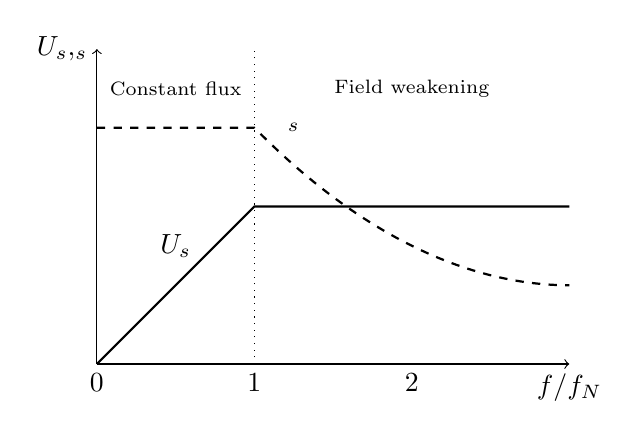
\begin{tikzpicture}
    % horizontal axis
    \draw[->] (0,0) -- (6,0) node[anchor=north] {$f/f_N$};
    % labels
    \draw	(0,0) node[anchor=north] {0}
    		(2,0) node[anchor=north] {1}
    		(4,0) node[anchor=north] {2};
    % ranges
    \draw	(1,3.5) node{{\scriptsize Constant flux}}
    		(4,3.5) node{{\scriptsize Field weakening}};
    % vertical axis
    \draw[->] (0,0) -- (0,4) node[anchor=east] {$U_s,\varPsi_s$};
    % nominal speed
    \draw[dotted] (2,0) -- (2,4);
    % Us
    \draw[thick] (0,0) -- (2,2) -- (6,2);
    \draw (1,1.5) node {$U_s$}; %label
    % Psis
    \draw[thick,dashed] (0,3) -- (2,3) parabola[bend at end] (6,1);
    \draw (2.5,3) node {$\varPsi_s$}; %label
    \end{tikzpicture}
  \caption{A tikz figure example}
  \label{fig:tikz}
\end{figure}

\chapter{Lorem Ipsum}
\lipsum[2-9]


\begin{acknowledgements}
\lipsum[2]
\end{acknowledgements}

\printbibliography[title=References,heading=bibintoc]

\clearpage % ensure all floats are processed
\processdelayedfloats
\clearpage


\begin{appendices}
\chapter{Versions}
\begin{description}
  \item[2019] 1st version by Zhenghao Yin, Takeuchi lab.
\end{description}


\chapter{Layout and Parameters}
Default parameters used in this template is shown in \ref{tab:text},\ref{tab:fig}.

\begin{table}
  \caption{Default layout}\label{tab:text}
  \begin{center}
    \begin{tabular}{|l|r|}
      \hline
      \verb+\textwidth+ & 424pt \\ \hline
      \verb+\textheight+ & 604pt \\ \hline
      \verb+\oddsidemargin+ & 0.5cm \\ \hline
      \verb+\evensidemargin+ & 0.5cm \\ \hline
      \verb+\topmargin+ & 0pt \\ \hline
      \verb+\headheight+ &12pt \\ \hline
      \verb+\headsep+ & 25pt \\ \hline
      \verb+\footskip+ & 30pt \\ \hline
    \end{tabular}
  \end{center}
\end{table}

\begin{table}
  \caption{Default parameters for graphs}\label{tab:fig}
  \begin{center}
    \begin{tabular}{|l|r|}
      \hline
      \verb+\textwidth+ & 424pt + 1cm \\ \hline
      \verb+\textheight+ & 604pt + 67pt \\ \hline
      \verb+\oddsidemargin+ & 0pt \\ \hline
      \verb+\evensidemargin+ & 0pt \\ \hline
      \verb+\topmargin+ & 0pt \\ \hline
      \verb+\headheight+ & 0pt \\ \hline
      \verb+\headsep+ & 0pt \\ \hline
      \verb+\footskip+ & 0pt \\ \hline
    \end{tabular}
  \end{center}
\end{table}
\end{appendices}


\end{document}

